% !Mode:: "TeX:UTF-8"

\chapter[绪论]{绪论}[Introduction]

\section{课题背景及意义}[Background and Significance]

\subsection{课题背景}[Background]

% 先写语义分析

% 树结构在语义表示方面的不足, 中英文都出现了语义图标注 (举例)

% 图分析的难点

让机器理解自然语言,是自然语言处理领域最根本也是最重要的问题之一。
要实现在语义层面上理解自然语言,自然语言处理领域的传统方法一般对文本进行自底向上的分词、词性标注、命名实体识别、句法分析,最后才能进行语义分析。
然而,由于中文严重缺乏形态变化,词类与句法成分没有严格的对应关系,导致中文句法分析的精度始终不高。
例如,在英文宾州句法树库(Penn Treebank, PTB)\cite{marcus-etal-1993-building}上目前句法分析准确率已经能达到95\%,而在中文宾州句法树库(Penn Chinese Treebank, CTB)\cite{xue-etal-2005-penn}上则只能达到88\% \cite{dozat-etal-2017-deep}。
为了解决这些问题,哈工大社会计算与信息检索研究中心结合中文重意合、在形式分析上有劣势的语言特点,于2011年在世界上最早提出了跨越句法分析直接进行语义依存分析的思路,并与北京语言大学邵艳秋教授合作标注了中文语义依存树语料库,用树结构融合依存结构和语义关系。

与句法结构相比,句子中词之间的语义关系往往更加复杂。
而传统句法分析中使用的树结构已经无法胜任对如此复杂的语义关系的刻画。
因此,研究者将目光聚集到约束更少的图结构上,希望用图结构来表示这些语义关系。
在英文上,Oepen等人在宾州句法树库的华尔街日报(Wall Street Journal,简称为WSJ)语料上,构建了三种不同标注规范的语义依存图,并于国际语义评测大赛SemEval 2014\cite{oepen-etal-2014-semeval}和SemEval 2015\cite{oepen-etal-2015-semeval}上组织了公开评测任务。
在中文上,哈工大社会计算与信息检索研究中心将中文语义依存树结构扩展为语义依存图,从而更全面地刻画句中词之间的语义关系,并在国际语义评测大赛SemEval 2016\cite{che-etal-2016-semeval}上组织了公开评测任务。
这些语义依存图语料库的构建,吸引了越来越多的研究者在语义依存分析领域开展研究,有力推动了该领域的发展。

与分词、词性标注、句法分析等历史悠久的研究课题相比,语义依存图分析算得上是一个新兴课题,无论是其基础分析方法,还是在不同情境下的应用,以至于如何利用它帮助其他自然语言处理任务,都有待深入探究。
以下从语义依存图分析方法、非规范文本上和多语言文本上的语义依存图分析以及利用语义依存图帮助其他自然语言处理任务四个方面简要阐述相应的研究背景。

1.\textbf{语义依存图分析方法}。
语义依存图分析器的设计,是该领域最基本也是最重要的问题。
得益于语义依存图与传统句法依存树的相似性,依存图的分析方法可以从大量的句法依存分析工作中借鉴经验。
但图结构在带来更全面的语义表示的同时,也给语义依存分析任务带来了巨大的挑战。
对于依存树结构,每个词只有一个父节点,而在依存图中,每个词可能有多个父节点,这给分析系统带来了很大的不确定性,从而增加了语义依存分析任务的难度。
这也是依存图分析器的设计中亟需解决的研究课题。

2.\textbf{非规范文本上的语义依存图分析}。
近期有研究表明,基于神经网络的模型尽管在情感分析\cite{zhang-etal-2019-generating}和文本蕴涵\cite{jin-etal-2020-isbert}等自然语言处理任务的标准数据集上取得了很高的精度,但在非规范文本上这些模型的性能会大大下降。
这一发现揭示了目前广泛应用的神经网络模型的脆弱之处,也加强了研究者们对模型鲁棒性的重视。
然而目前这类鲁棒性研究多集中于句子级分类任务上,神经网络模型在语义依存分析等结构化预测任务上的鲁棒性有待深入探究。

3.\textbf{多语言文本上的语义依存图分析}。
目前语义依存图分析的研究基本都集中在以中英文为代表的少数几种资源丰富的语言上,这是由于人工标注的语义依存图语料只存在于这几种语言上。
然而,对于世界上的大部分语言来说,语义依存图语料难以获取,且人工标注代价较高。
因此,如何充分利用现有人工标注的语料资源,以最小的代价实现对资源稀缺语言的语义依存图分析,也是研究者一直关注的问题。

4.\textbf{利用语义依存图帮助其他任务}。
语义依存图分析任务最重要的作用之一是为其他自然语言处理任务提供所需的语义信息。
然而,目前大多数该领域的研究仍集中在依存分析器的构建上。
此外,随着基于变换器的双向编码器表示模型(Bidirectional Encoder Representations from Transformers,简称BERT)\cite{devlin-etal-2018-bert}等预训练模型在自然语言处理各个任务上取得令人瞩目的成绩,句法依存树和语义依存图等人工定义的结构的必要性正面临质疑。
因此,在预训练语言模型大行其道的背景下,如何利用语义依存图帮助其他自然语言处理任务,也是一个重要的研究课题。


\subsection{课题意义}[Significance]

语义依存分析建立在依存理论基础上,是对语义的深层分析,具有形式简洁,易于理解和运用的优势。
其具体可分为两个阶段,首先是根据依存语法建立依存结构,即找出句子中的所有修饰词与核心词对,然后再对所有的修饰词与核心词对指定语义关系。
因此,语义依存分析可以同时描述句子的结构和语义信息。
与传统句法分析相比,语义依存图分析主要有以下三个优点。


\begin{figure}[htpb]
	\begin{center}
			\begin{dependency}[arc edge, arc angle=80, text only label, label style={above}]
				\begin{deptext} [row sep=0.6cm, column sep=.5cm]
					\ ROOT \& 早起 \& 使 \& 人 \&  健康 \\
				\end{deptext}
				\depedge{1}{3}{\color{black}Root}
				\depedge{3}{2}{\color{black}Exp}
				\depedge{3}{4}{\color{black}Datv}
				\depedge{3}{5}{\color{black}eResu}
				\depedge{5}{4}{\color{black}Exp}
				
				\depedge[edge below]{1}{3}{\color{black}root}
				\depedge[edge below]{3}{2}{\color{black}nsubj}
				\depedge[edge below]{3}{4}{\color{black}dobj}
				\depedge[edge below]{3}{5}{\color{black}dep}
			\end{dependency}
			%\caption{语义依存图(上方)与句法依存树(下方)对比示例}
			\bicaption[fig:sdg0]{}{语义依存图(上方)与句法依存树(下方)对比示例}{Fig.$\!$}{Example of semantic dependency graph (upper) and syntactic dependency tree (lower)}
	\end{center}
\end{figure}


首先,它不受到句法分析中树结构的限制,因此可以更全面地覆盖句中各个词之间的语义关系。
图\ref{fig:sdg0}给出了一个中文语义依存图和句法依存树对比的例子,在句子“早起使人健康”中,“人”同时作为“使”的与事者(Dative, Datv)和“健康”的当事者(Experiencer, Exp),这种关系在有树结构限制的句法标注中难以直接体现,但在语义依存图中则可以直接刻画出来。

其次,语义依存关系比句法依存关系更细化。
例如,“他吃苹果”和“他很高”中的“他”在句法依存分析中都是主语,但前一个句子中的谓词是他的动作,而后一个句子中的谓词描述的是他的特点,这二者的语义是有明显区别的。
因此在语义依存图中前一个“他”标注为施事者(Agent,Agt),后一个“他”标注为当事者(Experiencer,Exp)。
此外,句法依存关系中对句中多个谓词之间的关系没有明确划分。
而在语义依存关系中,定义了并列、条件、转折等详细的谓词间关系。

\begin{figure}[htb]
	\begin{center}
			\begin{dependency}[arc edge, arc angle=80, text only label, label style={above}]
				\begin{deptext} [row sep=0.4cm, column sep=.1cm]
					\ ROOT \& 张三 \& 昨天 \& 告诉 \&  李四  \& 一件 \& 事 \\
				\end{deptext}
				\depedge{1}{4}{\color{black}Root}
				\depedge{4}{2}{\color{black}Agt}
				\depedge{4}{3}{\color{black}Time}
				\depedge{4}{5}{\color{black}Datv}
				\depedge{4}{7}{\color{black}Cont}
				\depedge{7}{6}{\color{black}Quan}
			\end{dependency}
			\bicaption[fig:sdp0]{}{语义依存图示例}{Fig.$\!$}{Example of semantic dependency graph}
	\end{center}
\end{figure}

\begin{figure}[htb]
	\begin{center}
			\begin{dependency}[arc edge, arc angle=80, text only label, label style={above}]
				\begin{deptext} [row sep=0.4cm, column sep=.1cm]
					\ ROOT \& 昨天 \& , \& 张三 \&  将  \& 一件 \& 事 \& 告诉 \& 李四  \\
				\end{deptext}
				\depedge{1}{8}{\color{black}Root}
				\depedge{2}{3}{\color{black}mPunc}
				\depedge{7}{5}{\color{black}mPrep}
				\depedge{7}{6}{\color{black}Quan}
				\depedge{8}{2}{\color{black}Time}
				\depedge{8}{4}{\color{black}Agt}
				\depedge{8}{7}{\color{black}Cont}
				\depedge{8}{9}{\color{black}Datv}
			\end{dependency}
			\bicaption[fig:sdp1]{}{语义依存图示例}{Fig.$\!$}{Example of semantic dependency graph}
	\end{center}
\end{figure}


最后,语义分析可以跨越句子的表层结构直接获取深层语义表达的本质,它通过在句子结构中分析实词间的语义关系来直接回答句子中“谁在何时何地对谁做了什么”等问题。
以图\ref{fig:sdp0}中的中文句子“张三昨天告诉李四一件事”为例,通过语义依存分析,我们能获知“谁告诉李四一件事?”、“张三告诉谁一件事?”、“张三何时告诉李四一件事?”及“张三告诉李四什么?”等问题的答案。
另外,图\ref{fig:sdp1}中的句子“昨天,张三将一个秘密告诉李四。”虽然与图\ref{fig:sdp0}中的句子“昨天,张三将一件事告诉李四”表述形式不同,但含义相同,因此它们的语义依存结构相同。
因此语义依存分析能为问答系统、信息抽取、信息检索等对语义信息要求较高的任务提供很大帮助。
%因此语义依存分析可以解决问答系统、信息抽取、信息检索等任务中的“多句一意”情况。

总的来说,语义依存图分析打破了传统句法依存分析中的树结构,能更全面、直接地获取深层语义表示,提供了更加细粒度的语义关系,从而为需求语义信息的其他自然语言处理任务提供帮助。
从上述研究意义出发,本文围绕中文语义依存图分析任务,立足依存分析技术本身,深入探究在非规范文本和多语言文本上的语义依存图分析,最终利用语义依存图帮助其他自然语言处理任务,为语义依存图的应用提供了一种可能性。

\section{研究现状与分析}[Related Work]
本节介绍了与本文研究的语义依存图分析相关的各领域研究现状。
具体来说,本文首先介绍语义依存图分析的前身——句法依存分析的研究现状,然后介绍本文的主要研究目标——语义依存分析与句法依存分析的异同及其研究现状。
接着,针对非规范文本和跨语言语义依存分析任务,本文分别介绍了目前自然语言处理领域对神经网络模型鲁棒性的研究以及跨语言依存分析的方法和研究现状。
最后,本文介绍了现阶段以依存句法结构为代表的结构化信息在神经网络模型中应用的研究现状。

\subsection{句法依存分析}[Syntactic Dependency Parsing]
\label{sec:syntactic-dependency-parsing}

句法依存分析是语义依存图分析的前身,相对于刚起步的语义依存图分析,自然语言处理领域的研究者对句法依存分析已经有近二十年的研究。
得益于语义依存图与传统句法依存树的相似性,依存图的分析方法可以从丰富的句法依存分析工作中借鉴经验。
因此本文首先介绍传统句法分析领域的主要研究方法。

\begin{figure}[htb]
	\begin{center}
			\begin{dependency}[arc edge, arc angle=80, text only label, label style={above}]
				\begin{deptext} [row sep=0.4cm, column sep=.1cm]
					\ ROOT$_0$ \& 张三$_1$ \& 吃$_2$ \& 苹果$_3$ \\
				\end{deptext}
				\depedge{1}{3}{\color{black}root}
				\depedge{3}{2}{\color{black}nsubj}
				\depedge{3}{4}{\color{black}dobj}
			\end{dependency}
			\bicaption[fig:syntax-tree]{}{句法依存树示例}{Fig.$\!$}{Example of syntactic dependency tree}
	\end{center}
\end{figure}

如图\ref{fig:syntax-tree}中的例子所示,句法依存分析能够直接描述句子中词与词之间的句法关系,称为依存关系(Dependency Relations)。
两个词之间的依存关系用一条有向弧表示,其由核心词(head,或称为governer)指向修饰词(dependent,或称为modifier),核心词和修饰词之间的句法关系用弧上的标签表示。
例如,图\ref{fig:syntax-tree}中,“张三”是“吃”的主语,用标签“nsubj”表示。
根据定义,一棵句法依存树需要满足以下三个条件:(1)有且仅有一个根节点,该节点是其他所有节点的公共祖先节点;(2)每个词都有且仅有一个父节点;(3)将该依存树按词序排列,句中所有弧可以在句子的一边(上方或下方)表示且不存在交叉弧。
具体来讲,对于第一个条件,在实际应用中,一般会建立一个虚拟根节点“ROOT”指向句中的这个根节点,他们之间的关系为“root”。
第二个条件确保的所有的依存弧能组成一个完整的全连接树。
而第三个条件称为依存树的投射性(projectivity),它对于某些依存分析方法具有重要意义。

目前主流的依存句法分析方法主要可以分为以下两类:

1.\textbf{基于转移的方法}。
该方法由Yamada等人\cite{yamada-etal-2003-statistical}和Nivre\cite{nivre-2003-efficient}分别于2003年同时最先提出。
其核心思想是设计基于移进-规约的转移系统,通过一条转移动作序列,逐步生成句子的依存树。
具体来说,这类算法包括两部分,即转移系统和转移动作分类器。
转移系统一般由一个保存部分处理的句法依存结构的栈和一个保存尚未处理的词的队列组成。
转移动作一般包括移进和生成弧,前者将队列中的词移入栈中,后者则负责生成依存弧。
转移系统根据转移动作而改变,在每一步时,转移动作分类器根据当前的转移系统状态预测下一步的转移动作。
当队列为空,且栈中只有一棵依存树时,分析过程结束。
最初,研究者一般使用基于特征工程的统计机器学习方法实现转移动作分类器。
近年来,随着神经网络在自然语言处理领域的广泛应用,基于神经网络的模型逐渐替代了传统方法来实现此分类器。

表\ref{tbl:trans-seq-example}给出了图\ref{fig:syntax-tree}中对应的句法依存树的转移动作序列,展示了从初始状态经历一系列转移动作最终生成整个句法依存树的过程。
在表中,句子中的词用其下标数字表示,$\sigma$和$\beta$分别表示转移系统中的栈和队列,$E$表示已经生成的弧的集合。
该转移序列来自标准弧转移系统(Arc-Standard Transition System),其中定义了移进(Shift)、左弧(Left-Arc)和右弧(Right-Arc)三种转移动作。
其中移进动作将队列中第一个词移入栈顶。
而左弧和右弧动作则通过生成栈顶两个词之间的弧对以他们为根的两个子树进行合并,使其中一棵成为另一棵的子树。
初始状态下,栈中只有一个虚拟根节点,队列中保存句子中的所有词。
经过一系列转移动作,当队列为空且栈中只有一个以虚拟根节点为根节点的树时,转移序列结束,最终栈中的树就是算法生成的句法依存树。
值得注意的是,该方法要求目标依存树具有投射性。

\begin{table*}[thbp]
    \bicaption[tbl:trans-seq-example]{}{图\ref{fig:syntax-tree}中的句法依存树对应的转移动作序列示例}{Table$\!$}{Transition sequence example of the syntactic dependency tree in Fig.\ref{fig:syntax-tree}.}
	\vspace{0.5em}\centering\wuhao
	\begin{tabular}{C{3em}L{7em}R{4.5em}L{4em}L{9em}}
		\toprule[1.5pt]
		状态 & 转移动作 & $\sigma$ & $\beta$ & $E$ \\
		\midrule[1pt]
		$0$ & Initialization & $[0]$ & $[1, 2, 3]$ & $\emptyset $ \\
		$1$ & Shift & $[0, 1]$ & $[2, 3]$ &  \\
		$2$ & Shift & $[0, 1, 2]$ & $[3]$ &  \\
		$3$ & Left-Arc & $[0, 2]$ & $[3]$ & $E\ \cup\ \{1\leftarrow \textrm{nsubj}-2\}$ \\
		$4$ & Shift & $[0, 2, 3]$ & $[]$ &  \\
		$5$ & Right-Arc & $[0, 2]$ & $[]$ & $E\ \cup\ \{2- \textrm{dobj}\rightarrow3\}$ \\
        $6$ & Right-Arc & $[0]$ & $[]$ & $E\ \cup\ \{0- \textrm{root}\rightarrow2\}$ \\
		\bottomrule[1.5pt]
	\end{tabular}
\end{table*}

2.\textbf{基于图的方法}。
该方法由McDonald等人\cite{mcdonald-etal-2005-online}与2005年最先提出。
其核心思想是将依存分析视为在有向全连接图中寻找最大生成树(Maximum Spanning Tree)的问题。
具体来说,这类方法将一棵句法依存树视为若干子树(subtree)的集合,因而一棵句法依存树的分值就可以分解为这些子树的分值之和。
这类方法首先计算各个子树的分值,然后使用动态规划算法进行解码,求得使整个句法依存树分值最大的子树组合。
算法中使用的子树可以由一条弧组成,这时该方法称为一阶算法。
同理,若基本子树结构由两条弧组成,则称为二阶算法。\cite{carreras-2007-experiments}
随着阶数的增加,算法的复杂度也逐渐提升。
另一方面,在计算子树分值时,最初一般采用基于特征工程的统计机器学习方法。
此后随着神经网络在自然语言处理中的广泛应用,基于神经网络的模型也被用于预测子树分值。

\subsection{语义依存图分析}[Semantic Dependency Graph Parsing]
\label{sec:sdp}

为了表示比句法结构更复杂的语义结构,自然语言处理领域的研究者在探索中逐渐尝试用表示能力更强的图结构来代替传统的树结构。
根据语义图中的节点与句中词之间的关系,现有的语义图语料可以分为锚定(anchored)的和非锚定(unanchored)的两类。
第一类锚定的语义图特点为语义图中每个节点都与句子中的词一一对应,因此可以认为语义关系是直接标注在句中词与词之间的。
而第二类非锚定的语义图特点为语义图中的节点与句子中的词没有明确对应关系。

非锚定的语义图中最具代表性和影响力的是抽象语义表示(Abstract Meaning Representation,简称为AMR)。\cite{banarescu-etal-2013-abstract}
由于其语义图中的节点与句子中的词没有严格的对应关系,AMR具有较强的抽象能力,在获取不同表达形式的句子的相同语义内核方面具有一定优势。
但语义图节点与句中词关系的去相关化,也为AMR的分析和应用带来了巨大的挑战。

锚定的语义图中最具代表性的则是语义依存图,也是本文的主要研究内容。
相对于非锚定的语义图,语义依存图中的语义关系直接标注在句中的词之间,这大大降低了语义依存图的理解难度。
同时,得益于语义依存图与传统的句法依存树在结构上的相似性,无论是语义依存图的分析方法还是应用途径,都能从句法依存分析领域的大量研究中获取经验和灵感。
针对本文主要研究内容,本节主要介绍语义依存图分析领域的研究现状。
在结构上,语义依存图与句法依存树的主要区别在于句法依存树中每个词有且只能有一个父节点,而语义依存图中允许一个词拥有多个父节点。
此外,多父节点词的出现,也破坏了传统句法依存树的投射结构。
也就是说在语义依存图中,存在投射句法依存树中没有的交叉弧,这使得句法分析中的很多方法无法直接应用到语义依存图分析中。
因此,现有的语义依存图分析方法基本延续了句法依存分析中的基于转移的和基于图的两类方法,并将研究重点集中在如何解决上述的多父节点词问题上。

针对基于转移的方法,Du等人对句法依存树的转移系统进行修改\cite{du-etal-2014-peking},增加了交换(swap)动作,其作用是交换栈顶和队列中的第一个词。
这一动作解决了语义依存图中存在交叉弧的问题。
此外,他们还修改了生成弧的转移动作,在生成两个词之间的弧之后,不再从转移系统中删除其中的子节点,而是增加了一个额外的弹栈(pop)动作用于删除已经找到所有父节点和子节点的词。
这一改动使得他们的转移系统能为一个词生成多个父节点。
通过对转移系统的改动,该方法成功实现了对语义依存图的分析。
大部分基于转移的依存图分析方法\cite{sagae-tsujii-2008-shift,titov-etal-2009-online}也与该方法类似,都将重点放在对转移系统的修改上,而在另一个重要模块——转移动作分类器上沿用了传统的基于特征工程的统计机器学习方法。

针对基于图的方法,Almeida等人在句法依存树的二阶算法的子树结构中加入依存图特有的子树结构。\cite{martins-almeida-2014-priberam}
例如加入由一个词与其两个父节点之间的两条弧组成的子树。
通过这些依存图特有的子树结构,他们的算法将传统基于图的依存树分析算法无法覆盖的依存图子结构纳入考虑中,然后将依存图解码问题视为全局优化问题,采用对偶分解(dual decomposition)算法对其进行求解。

\subsection{非规范文本依存分析}[Dependency Parsing on Informal Texts]
\label{sec:chapter1-informal}

近年来,神经网络模型在语音识别、计算机视觉和自然语言处理等领域取得了重大成功。
然而,计算机视觉领域的研究者首先发现,在神经网络模型的输入中加入微小的扰动,会使其产生误判,从而导致性能大大下降。\cite{akhtar-etal-2018-threat}
这种扰动在计算机视觉领域一般是指对输入图像加入噪点。
这种噪点对于人类来说几乎是难以察觉的,但却能显著影响神经网络模型的判断。
这一发现加强了各领域的研究者对神经网络模型鲁棒性的重视程度,也引发了一系列相关研究。
随后,自然语言处理领域的研究者也开展了对神经网络鲁棒性的研究。\cite{zhang-etal-2020-adversarial}
在自然语言处理领域,输入的扰动则变为了对输入文本的修改,而这种修改也需要使得人类难以察觉。
从另一个角度来说,自然语言处理领域的模型鲁棒性研究,也可以理解为探索与传统的由规范文本组成的数据集相对应的非规范文本上的模型的表现。
本节首先介绍自然语言处理领域的神经网络模型,然后介绍该领域内研究者对神经网络模型在非规范文本上的多个任务的鲁棒性研究现状。

\subsubsection{自然语言处理领域的神经网络模型}

在自然语言处理领域中,神经网络模型的一个重要特征就是使用了连续、低维、稠密的词向量(word embedding)代替了传统统计机器学习方法中的离散、高维的符号表示。
因此本节从词向量的角度分别介绍自然语言处理领域中广泛使用的两类神经网络模型:基于固定词向量的模型和基于上下文相关词向量的模型。

1.\textbf{基于固定词向量的模型}。
在神经网络模型被应用于自然语言处理领域的早期阶段,固定词向量因为有效解决了离散特征表示维度过高造成的“维度灾难”问题(Curse of Dimensionality)而占有重要地位。
与传统方法中离散特征表示需要领域专家设计特征模板不同,固定词向量一般是通过基于神经网络的特征学习(Representation Learning)获取的。
固定词向量中最具代表性的是Mikolov等人于2013年提出的Word2vec算法\cite{mikolov-etal-2013-distributed}。
其中包括两个模型,分别是连续词袋模型(Continuous Bag-of-Words Model,简称CBOW)和跳跃文法模型(Skip-gram Model),如图\ref{fig:word2vec}所示。

\begin{figure}[htbp]
    \centering
    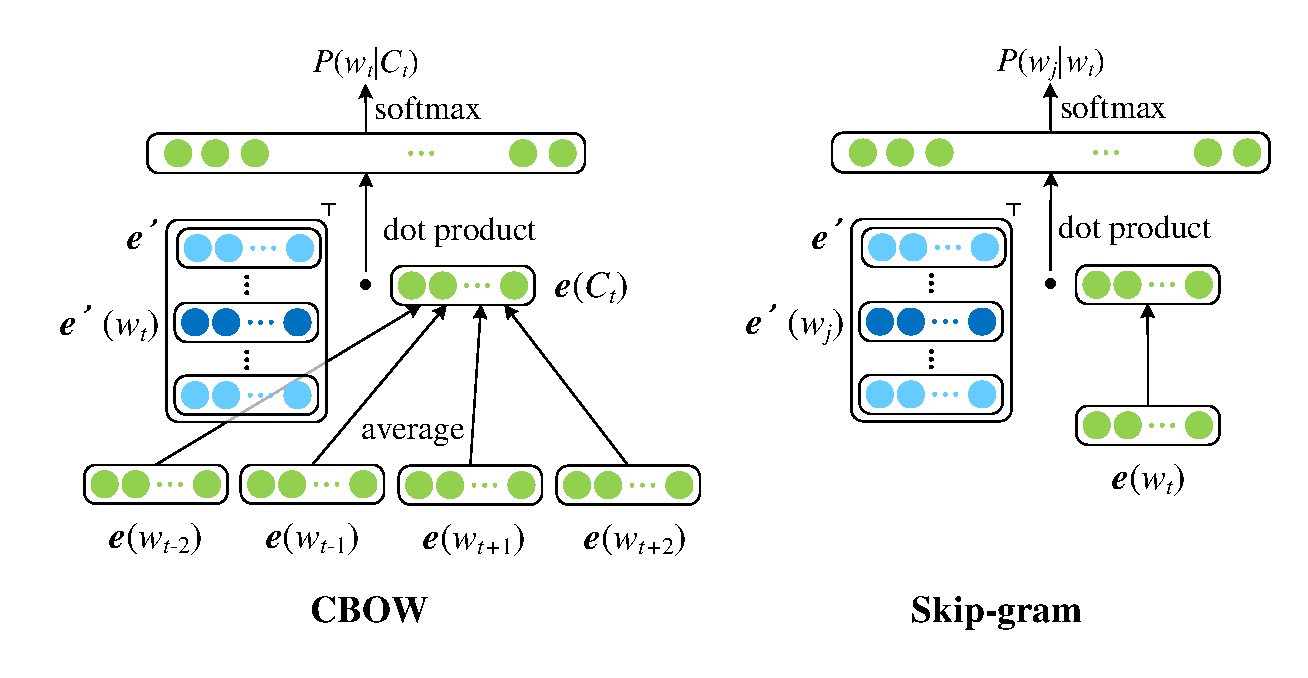
\includegraphics[width=0.95\textwidth]{figures/word2vec.pdf}
    \bicaption[fig:word2vec]{}{连续词袋模型(左)和跳跃文法模型(右)}{Fig.$\!$}{CBOW model (left) and Skip-gram model (right)}
\end{figure}

CBOW模型的核心思想是用一个词的上下文预测该词。
形式化地,给定一个目标词$w_t$及其上下文$C_t=\{w_{t-n},\dots,w_{t-1},w_{t+1},\dots,w_{t+n}\}$。
对于每个词$w_j$,模型中分别有输入词向量$\bm{e}(w_j)$和输出词向量$\bm{e}'(w_j)$作为其表示,其中输入词向量$\bm{e}(w_j)$是模型要学习的词向量。
该模型首先计算$w_t$上下文的词向量平均值$\bm{e}(C_t)=\frac{1}{|C_t|}\sum_{w_j\in C_t}\bm{e}(w_j)$,然后计算词$w_t$出现在上下文$C_t$中的概率:
\begin{equation}
    P(w_t|C_t)=\frac{\exp(\bm{e'}(w_t)^{\top}\bm{e}(C_t))}{\sum_{w'\in \mathbb{V}}\exp(\bm{e'}(w')^{\top}\bm{e}(C_t))}
\end{equation}
其中$\mathbb{V}$表示模型中的词表,而模型最终优化目标为最大化整个训练数据集上的平均对数概率:
\begin{equation}
    \frac{1}{T}\sum_{t=1}^{T}\log P(w_t|C_t)
\end{equation}
其中$T$表示训练集中的样本个数。

相对的,Skip-gram模型则用中心词$w_t$预测上下文$C$中的每个词$w_j$:
\begin{equation}
    P(w_j|w_t)=\frac{\exp(\bm{e'}(w_j)^{\top}\bm{e}(w_t))}{\sum_{w'\in \mathbb{V}}\exp(\bm{e'}(w')^{\top}\bm{e}(w_t))}
\end{equation}
其最终优化目标为最大化整个训练集上的平均对数概率:
\begin{equation}
    \frac{1}{T}\sum_{t=1}^{T} \sum_{w_j\in C_t} \log P(w_j|w_t)
\end{equation}

以Word2vec为代表的的固定词向量学习方法,为自然语言处理领域提供了新的词表示方式,在神经网络模型中发挥了重要作用,有效地提高了大量自然语言处理任务上的性能。

2.\textbf{基于上下文相关词向量的模型}。
虽然固定词向量有效解决了维度灾难问题,但其是建立在每个词只有一个表示向量的假设下的。
然而在自然语言中存在大量的一词多义现象,一个单独的词向量往往无法很好地表示多义词的所有含义。
为解决这一问题,研究者逐渐开始使用上下文来动态的获取词的表示向量。
这一思想起源于自然语言处理中的语言模型,即根据前文预测下一个词。
Bengio等人早在2005年就提出了一种利用有限窗口中的\cite{bengio-etal-2003-neural}前文预测下一个词的语言模型。
从后来的Word2vec算法中也能看到这一思想的影子。
但在很长一段时间中,研究者都只使用这种方法获取的固定的静态词向量,然后用于其他任务。

\begin{figure}[htbp]
    \centering
    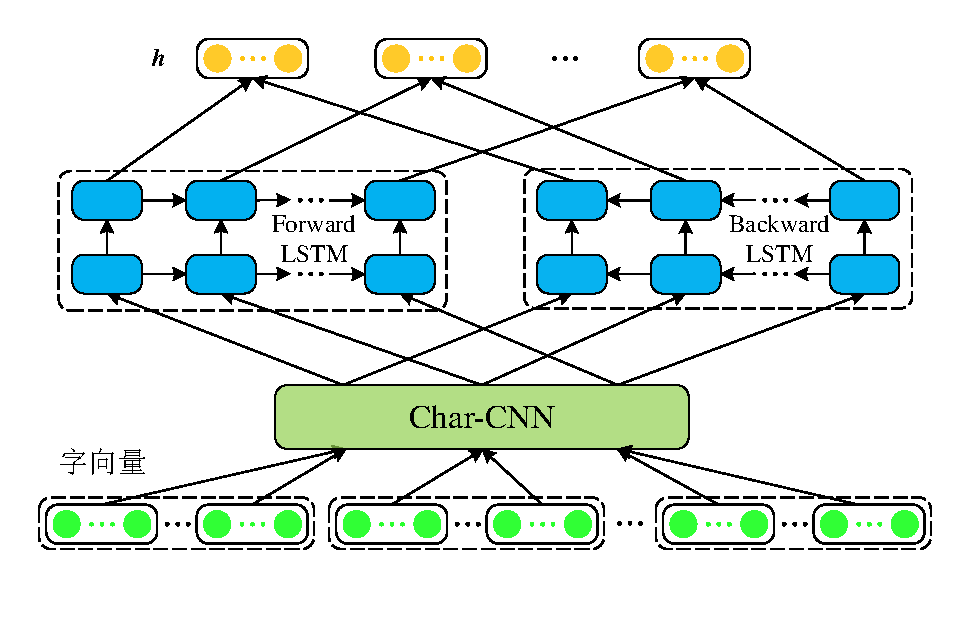
\includegraphics[width=0.7\textwidth]{figures/elmo.pdf}
    \bicaption[fig:elmo]{}{ELMo模型结构}{Fig.$\!$}{ELMo model architecture}
\end{figure}

直到Peters等人于2018年提出了基于语言模型的上下文相关词向量(Embeddings from Language Models,简称ELMo)\cite{peters-etal-2018-deep}。
如图\ref{fig:elmo}所示,该方法使用基于双向长短时记忆网络(Long-Short Memory Network,简称LSTM)的语言模型为文本中的每个词生成基于上下文的动态词向量,通过这种方式,同样的词在不同上下文中会获得不同的向量表示,从而有效缓解了一词多义问题。
ELMo的学习目标还是语言模型,即根据上文预测下一个词,但其中使用了从左到右和从右到左两个方向的语言模型,从而使最终的动态词向量能同时获取上下文的信息。
具体来说,对于一个句子$\{w_1,\dots,w_n\}$,ELMo的最终优化目标为两个方向的语言模型的对数似然之和:
\begin{equation}
    L= \log(P(w_i|w_1,\dots,w_{i-1})) + \log(P(w_i|w_{i+1},\dots,w_{n}))
\end{equation}

值得注意的是,为了缓解不在词表中的词的问题,ELMo采用了字向量代替词向量作为输入,然后用基于字的卷积神经网络(Convolutional Neural Network,简称CNN)获取词的上下文无关表示。
接着将其输入到多层双向LSTM中,获取上下文相关的表示,以从左到右的语言模型为例,第$i$个词在第$k$层LSTM的表示为:
\begin{equation}
    \overleftarrow{\bm{h}}_i^{(k)} = \overleftarrow{\textrm{LSTM}}^{(k)}(\overleftarrow{\bm{h}}_1^{(k-1)},\dots,\overleftarrow{\bm{h}}_i^{(k-1)})
\end{equation}
其中$\overleftarrow{\bm{h}}_i^{(0)}=\bm{v}_i$为上述用CNN获取的上下文无关词向量。
假设LSTM共有$L$层,则最终为第$i$个词输出的上下文相关词向量为$L$层隐层状态的加权平均:
\begin{equation}
    \textrm{ELMo}_i = \gamma \sum_{k=0}^{L}s_k \cdot (\overleftarrow{\bm{h}}_i^{(k)}\oplus\overrightarrow{\bm{h}}_i^{(k)})
\end{equation}
其中$\gamma$为可学习参数,可以在应用在其他任务时动态的学习。

ELMo在命名实体识别\cite{tjong-kim-sang-de-meulder-2003-introduction}、情感分析\cite{socher-etal-2013-recursive}、文本蕴涵\cite{bowman-etal-2015-large}、阅读理解\cite{rajpurkar-etal-2016-squad}、语义角色标注\cite{pradhan-etal-2013-towards}和共指消解\cite{pradhan-etal-2012-conll}等六个数据集上取得了当时最优结果,有效证明了上下文相关词向量的重要性,也引起了许多研究者对此的兴趣。

紧随ELMo的脚步,Radford等人在2018年提出使用单向Transformer代替LSTM对语言模型进行建模,称为生成式预训练模型(Generative Pre-Training,简称GPT)\cite{radford-etal-2018-improving}。
除了上述区别外,GPT相比ELMo的另一特点是在目标任务上对预训练的语言模型进行精调参数(fine tuning)。
这种方法进一步提升了模型的性能,并被很多后续的工作所采用。

\begin{figure}[htbp]
    \centering
    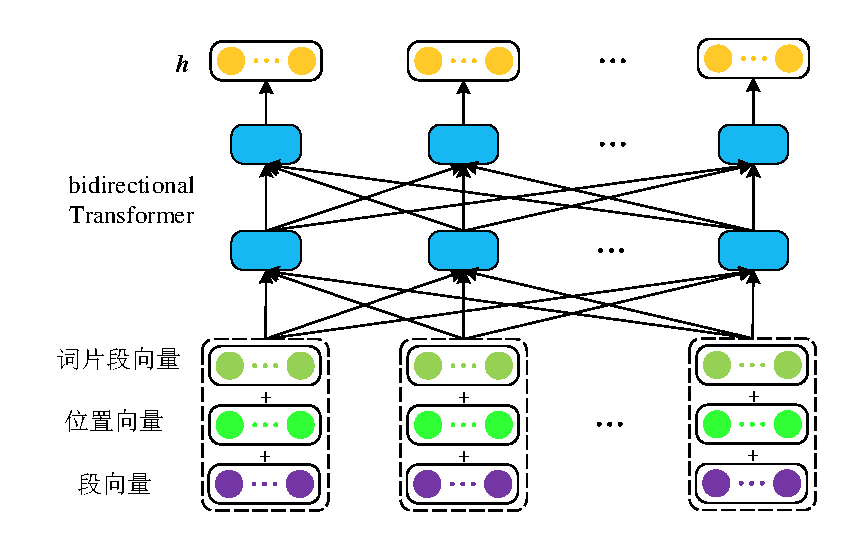
\includegraphics[width=0.7\textwidth]{figures/bert.pdf}
    \bicaption[fig:bert]{}{BERT模型结构}{Fig.$\!$}{BERT model architecture}
\end{figure}

在GPT和ELMo的基础上,Devlin等人于2018年提出了基于变换器的双向编码器表示模型(Bidirectional Encoder Representations from Transformers,简称BERT)\cite{devlin-etal-2018-bert},同时建模目标词的上下文。
他们提出遮盖语言模型(masked language model)代替传统单向语言模型作为学习目标,通过将目标词遮盖然后用其上下文预测该词实现了同时利用左右两个方向的上下文信息。
此外,他们还提出了预测下一个句子任务(next sentence prediction),将两个句子连接起来并预测第二个句子是否是第一个的后续句子。
与GPT相同,由于两个学习目标都不需要标注信息,BERT也是在大规模的未标注文本上进行预训练,然后再在目标任务上进行精调参数。
如图\ref{fig:bert}所示,为了缓解不在词表中的词的问题,BERT用词片段向量代替了词向量。
此外,与有向的LSTM不同,BERT采用的Transformer结构是全连接的,无法有效表示文本中词的位置信息。
为解决这一问题,BERT在输入向量中加入了位置向量用来表示输入的每个词片段的位置。
最后,由于BERT的训练过程中要将两个句子拼接起来,其在输入中额外加入了段向量用来区分当前词是属于第一句还是第二句的。

BERT在11项自然语言处理任务上取得了令人瞩目的大幅度性能提升,并以其强大的表示能力吸引了众多研究者的目光,开启了自然语言处理领域的预训练时代。
在BERT出现之前,自然语言处理领域中的各个任务一般都有针对它们的特点专门设计的各不相同的神经网络。
随着BERT之后越来越多预训练模型的出现,其渐成为了大部分任务的通用解决方法,研究者们逐渐趋向于使用大规模无标注数据在某些人工定义的任务上先对模型进行预训练,然后再针对目标任务进行精调参数。

\subsubsection{非规范文本上神经网络模型的鲁棒性}
\label{sec:chapter1-informal-text-attack}

尽管神经网络模型在自然语言处理领域取得了巨大的成功,但近期越来越多研究表明,神经网络模型在非规范文本上的鲁棒性存在明显问题。
这类研究一般采用对抗样本攻击的方式,具体来说,就是设计算法生成使目标模型产生误判的非规范文本,也即对抗样本。
根据攻击者对目标系统的了解程度,对抗样本攻击可以大致分为白盒攻击和黑盒攻击两类。
在白盒攻击情境下,攻击者能获取目标系统的所有信息,包括模型结构,参数及权重值等。
而在黑盒攻击情境下,攻击者仅能用对目标系统查询的方式,通过输入观察输出结果。
本节分别介绍自然语言处理领域中的白盒攻击和黑盒攻击。

1.\textbf{白盒攻击}。
由于在白盒攻击情境下攻击者能看到目标模型的参数和权重,这类攻击方法一般采用基于梯度的方法,寻找使目标模型的损失函数最大化的对输入文本的修改方案。
例如,Ebrahimi等人在2018年提出了HotFlip方法。\cite{ebrahimi-etal-2018-hotflip}
该方法提出了对输入进行字母级别的替换、插入和删除等修改,然后通过计算目标模型损失函数针对输入的独热表示(one-hot representation)的梯度,来搜索使损失函数最大化的修改。
该方法被用于攻击文本分类任务上的字级别神经网络模型,并证明了仅仅修改几个字母就能大大降低该模型的分类准确率。
Michel等人在2019年使用了类似的基于梯度的方法\cite{michel-etal-2019-evaluation},用词级别的替换代替了字母级别的修改,并在机器翻译任务上验证了他们提出的攻击方法的有效性,同时也证明了基于神经网络的机器翻译模型在非规范文本上鲁棒性较低。


2.\textbf{黑盒攻击}。
与白盒攻击相比,黑盒攻击情境与现实场景更接近,攻击者只能观测到模型的输入文本和输出的预测结果。
因此这类攻击方法一般以输入文本修改前后输出的预测结果的准确率作为依据,搜索使得预测结果准确率最低的修改。
例如,Alzantot等人在2018年提出针对文本分类任务的基于词替换的黑盒攻击方法\cite{alzantot-etal-2018-generating}。
该方法首先用预训练词向量计算句中词的$k$近邻作为其候选替换词,然后采用遗传算法(genetic algorithms)搜索其中使错误类别概率最高的候选词对原词进行替换。
值得注意的是,相比于前面介绍的无目的的对抗样本攻击,该方法能够通过最大化攻击者设定的目标类别的概率实现控制目标模型对对抗样本预测的类别的目的。
该方法被应用于攻击情感分析和文本蕴涵任务上的神经网络模型,并取得了很高的攻击成功率。
前面介绍的攻击方法选取的目标模型,基本都是传统的LSTM模型。
Jin等人在2020年将BERT模型也纳入了攻击的目标\cite{jin-etal-2020-isbert},采用了类似的词级别替换方法,按照句中词的重要性顺序搜索使正确类别置信度降低最多的替换。
他们在文本分类和文本蕴涵任务上证明了自然处理领域常用的CNN、LSTM和BERT模型在面对对抗样本攻击时,性能都会极大下降。

值得注意的是,前面介绍的攻击方法,无论是白盒攻击还是黑盒攻击,应用的任务基本都是文本分类任务或机器翻译这种生成任务。
很少有工作将目光放在自然语言处理领域中另一类非常重要的任务——结构化预测任务。
本文的主要研究的语义依存图分析也属于结构化预测任务,这类任务的特点是模型需要预测的是一系列而非一个标签,因而其难度也远大于文本分类这种只需要预测一个标签的任务。
而作为为其他任务提供重要语义信息的底层任务,语义依存分析器在非规范文本上的性能,或者说其鲁棒性,也是很重要的。
因此针对此问题的研究,以及在此基础上如何有效提高语义依存分析器鲁棒性的研究,都是本领域很有意义的研究课题。

\subsection{跨语言依存分析}[Cross-Lingual Dependency Parsing]

在世界上的大部分语言中,无论是语义依存图,还是其前身句法依存树,人工标注资源都非常稀缺。
在这种情况下,跨语言依存分析的目标就是最大限度地利用现有的人工标注资源,实现资源稀缺语言上的依存分析。
该任务有两个重要组成部分,分别是多语言数据和跨语言分析方法。
在科研情境下,多语言数据最重要的作用之一是提供一个可以评价跨语言分析模型性能的平台。
需要注意的是在研究中一般选择的语言可能并不是真正的资源十分稀缺的语言,而是用有人工标注资源的语言来模拟现实场景中的资源稀缺语言,从而对跨语言分析模型进行评价。
而在现实应用中,真正资源稀缺的语言上可能完全没有人工标注资源。
无论从人工标注资源的规模还是跨语言分析方法的研究上讲,相比于刚起步的语义依存图分析,句法依存分析领域都是大大领先的。
因此,本节先介绍句法依存分析领域的跨语言分析方法,然后介绍句法依存分析和语义依存图分析两个领域现有的多语言人工标注资源。

\subsubsection{跨语言依存分析方法}

在跨语言依存分析中,一般将有人工标注资源的语言称为源语言,而将没有人工标注资源,或者资源较少的语言称为目标语言。
其目标就是利用源语言数据来帮助目标语言的依存分析。
现有的跨语言依存分析方法主要可以分为以下三类:

1.\textbf{基于树库翻译的方法}。
这类方法的主要思想是将现有的源语言依存树库通过翻译的方式转换为目标语言的树库,然后利用该转换的树库在目标语言上训练分析器。
Tiedemann等人在2014年提出了基于树库翻译的跨语言依存分析方法\cite{tiedemann-etal-2014-treebank}。
他们采用了逐词翻译的方式,只允许一一对应的翻译,这样在将源语言上的句子翻译成目标语言之后,源语言上的依存标注就能很轻易地通过词的一一对应关系转移到目标语言上,从而获取目标语言上的标注资源。
这种方法的优点是不需要对分析模型做任何修改,其后来也被应用到跨语言语义角色标注等任务上\cite{fei-etal-2020-cross}。


2.\textbf{基于跨语言词向量的方法}。
这类方法是跨语言迁移学习里应用更广泛的一类方法,其核心思想是将源语言和目标语言的词向量投射到同一语义空间获取跨语言词向量,然后用跨语言词向量在源语言标注资源上训练模型。
这样在对目标语言的句子进行分析时,只要也使用跨语言词向量作为输入,就可以直接使用前面在源语言上训练的模型。
根据描述可以发现,这类方法中最核心的就是如何获取高质量的跨语言词向量。
Guo等人\cite{guo-etal-2015-cross}于2015年提出使用平行语料中获取的词对齐信息将源语言上的单语固定词向量投射到目标语言,从而获取跨语言词向量,并使用该词向量在跨语言句法依存分析任务上取得了较好结果。
此后,他们又在2016年提出一种对CBOW算法的修改使其能够直接训练跨语言词向量\cite{guo-etal-2016-representation}。
具体来说,他们在CBOW算法的有限窗口上下文中在源语言上下文的基础上,还加入了目标语言的上下文,即同时用多个语言的上下文预测中心词。
该方法获得的跨语言词向量在跨语言句法依存分析任务上取得了比上述方法更好的结果。

前面介绍的两种方法都是基于传统固定词向量的,在BERT被提出后,又出现了一批上下文相关的跨语言词向量\cite{conneau-etal-2019-cross,conneau-etal-2020-unsupervised},其中比较有代表性的有多语言BERT。
该模型使用了与BERT完全相同的模型结构,只是在训练时使用了来自一百多种语言的大规模无标注语料。
与BERT在很多任务上的表现类似,该模型在跨语言的依存分析上也取得了当时最好的结果\cite{kondratyuk-etal-2019-languages}。

3.\textbf{基于多任务学习的方法}。
这类方法也是跨语言迁移学习中应用很广泛的一类方法,其核心思想是通过共享神经网络的一部分参数,达到不同语言上的训练目标互相帮助的目的。
Guo等人\cite{guo-etal-2016-universal}于2016年提出一套多任务学习框架,在源语言和目标语言上使用相同的基于LSTM的句法分析模型,并共享其中一部分参数,同时在两个语言上进行训练,取得了较好结果。
需要注意的是,由于需要在源语言和目标语言上同时训练,这类方法需要源语言和目标语言上都有人工标注资源。
但通过与第一种树库翻译方法的结合,该方法也能实现只使用源语言标注资源进行学习。

\subsubsection{多语言句法依存及语义依存数据}

作为自然语言处理领域一个重要且传统的研究课题,句法依存分析领域的人工标注数据比语义依存图分析丰富很多,在以英文、中文等语言为代表的被广泛使用的语言上都有高质量的人工标注的句法树库。
在2006年\cite{buchholz-marsi-2006-conllx}和2007年\cite{nivre-etal-2007-conll}举办的两届CoNLL国际评测上,来自中文、英文、捷克语、阿拉伯语等十余种语言的句法树库被用于评价各参赛队伍的句法分析模型。
但这些来自各个语言的树库有着各自不同的句法关系定义和标注规范,这给跨语言依存分析带来了巨大的阻碍。
Mcdonald等人于2013年提出了多语言通用依存(universal dependencies)分析的思想\cite{mcdonald-etal-2013-universal}。
他们设计了一套适用于多种语言的句法关系和标注规范,并在德语、英语、瑞典语、西班牙语、法语和韩语等6种语言上依照这套规范进行了人工标注,为研究者提供了一套高质量的多语言通用依存树库,在依存分析领域造成了较大影响。
从2016年起,Nivre等人延续了多语言通用依存分析的思想,并着手构建更多语言的通用依存树库。
在2016年,跨语言通用依存树库的1.0版本\cite{nivre-2016-etal-universal}中已有33种语言的通用依存树库。
其中有的是人工标注的,有的是将各语言中已有的树库按照规则转换后再进行人工校对获得的。
接下几年中,随着该领域内越来越多研究者的加入,该项目下的语言和树库数量快速增多。
到2020年,跨语言通用依存树库的2.0版本\cite{nivre-etal-2020-universal}中已有90种语言的通用依存树库。
该项目至今仍然在不断更新中,跨语言通用依存树库最新的2.8版本中已经有114种语言的202个通用依存树库了。

相比于句法分析领域,语义依存图分析领域的人工标注数据则要少得多。
现存的大规模人工标注数据只有SemEval 2015任务18\cite{oepen-etal-2015-semeval}发布的DELPH-IN MRS-Derived Bi-Lexical Dependencies(DM)、Enju Predicate–Argument Structures(PAS)和Prague Semantic Dependencies(PSD)三种标注规范的数据集,以及SemEval 2016任务9\cite{che-etal-2016-semeval}发布的中文语义依存图数据集。
其中DM、PAS和PSD均有在英文上的标注数据,另外PAS还有一部分是在捷克语上进行标注的,而PSD还有一部分是在中文上标注的。

与已经有近十年发展时间的跨语言通用依存树库相比,语义依存图分析领域的人工标注数据的数量是十分稀少的,并且在很长一段时间内是很难追上的。
而且相比于树结构的句法依存树,由于语义依存图的标注过程中要考虑到更多的词和词之间的语义关系,其标注难度和成本都要大于句法依存树。
这也使得在语义依存图分析领域构建这样大规模的多语言人工标注资源成为了一件几乎不可能实现的任务。
但在看清这一点的同时,我们也应该注意到,由于句法依存树与语义依存图的相似性,跨语言通用依存树库就是现存的最好的跨语言人工标注资源。
因此如何利用跨语言通用依存树库中大规模的人工标注资源来帮助跨语言语义依存图分析,成为该领域需要重点解决的问题。

\subsection{结构化信息在神经网络模型中的应用}[Application of Structural Information in Neural Models]

以句法依存树为代表的结构化信息,在传统的神经网络模型中被广泛用于获取句子信息。
例如,Socher等人早在2011年就提出了递归神经网络(Recursive Neural Network,简称RecNN)\cite{socher-etal-2011-parsing},用于按照给定的句法结构对文本进行编码。
为了解决RecNN训练过程中出现的梯度消失(gradient vanish)和梯度爆炸(gradient explode)问题\cite{bengio-etal-1994-learning},Tai等人于2015年将长短时记忆的思想引入RecNN,提出了树结构LSTM(Tree-LSTM)\cite{tai-etal-2015-improved}。

随着以BERT为代表的预训练模型逐渐在自然语言处理领域占据主流地位,其强大的表示能力使得结构化信息的作用开始受到质疑。
有一系列针对BERT中蕴涵的信息的探测(probing)工作发现BERT中已经隐含了部分句法信息。
例如,Hewitt等人\cite{hewitt-manning-2019-structural}设计了一个计算BERT经过线性映射之后不同词之间距离的方法,证明了BERT中隐含了句子中的词在句法依存树上的距离信息。
而Jawahar等人\cite{jawahar-etal-2019-bert}和Lin等人\cite{lin-etal-2019-open}在探测工作中都发现,BERT的较低层的表示隐含更多句法信息,而较高层的的表示隐含更多语义信息。

尽管结构化信息在预训练时代的必要性受到了质疑,仍然有一系列工作在尝试将句法树等结构化信息与预训练模型进行结合。
例如,Fei等人\cite{fei-etal-2020-retrofitting}于2020年提出一种基于多任务学习的方法,在训练目标任务的同时预测句中词在句法树中的距离,从而隐式地将句法信息融入预训练模型中。
他们在命名实体识别、情感分类、关系分类等任务上测试了该方法,并取得了较明显的性能提升。
Munir等人\cite{munir-etal-2021-adaptive}于2021年提出一种使用Tree-LSTM和CNN将句法信息融入BERT顶层输出的方法,并将其应用到语义角色标注任务上,取得了较好的结果。

在语义相关的结构化信息应用上,Zhang等人\cite{zhang-etal-2020-semantics}于2020年提出将语义角色标注标签转化为表示向量,与从BERT中获取的表示向量合并,从而将语义角色标注信息融入BERT表示。
他们将该方法应用于文本分类、自然语言推理和语义相似性任务上,并取得了明显的性能提升。
Wu等人\cite{wu-etal-2021-infusing}于2021年提出使用图卷积网络(Graph Convolutional Network,简称GCN)将语义依存信息融入BERT顶层输出中,并在文本分类、自然语言推理和语义相似性任务上验证了该方法的有效性。

总的来说,目前关于如何利用语义依存图等结构化信息增强预训练模型表示能力的探索仍处于初步阶段,还有待于深入研究。

\section{本文的研究内容及章节安排}[Contents and Chapter Arrangement of the Thesis]

本文围绕中文语义依存图分析开展一系列研究工作。
从语义依存图分析方法本身入手,系统深入地探究了非规范文本和多语言文本上的语义依存图分析,并最终利用语义依存图有效帮助了其他自然语言处理任务。
在这几项研究内容中,语义依存图分析方法是首先需要解决的问题,也是支撑其他任务的基石。
在此基础上,我们探究了在非规范文本和多语言文本上的语义依存图分析,使语义依存图分析技术能适用于更多场景。
最后,我们研究了利用语义依存图帮助其他自然语言处理任务的方法。

\begin{figure}[htbp]
    \centering
    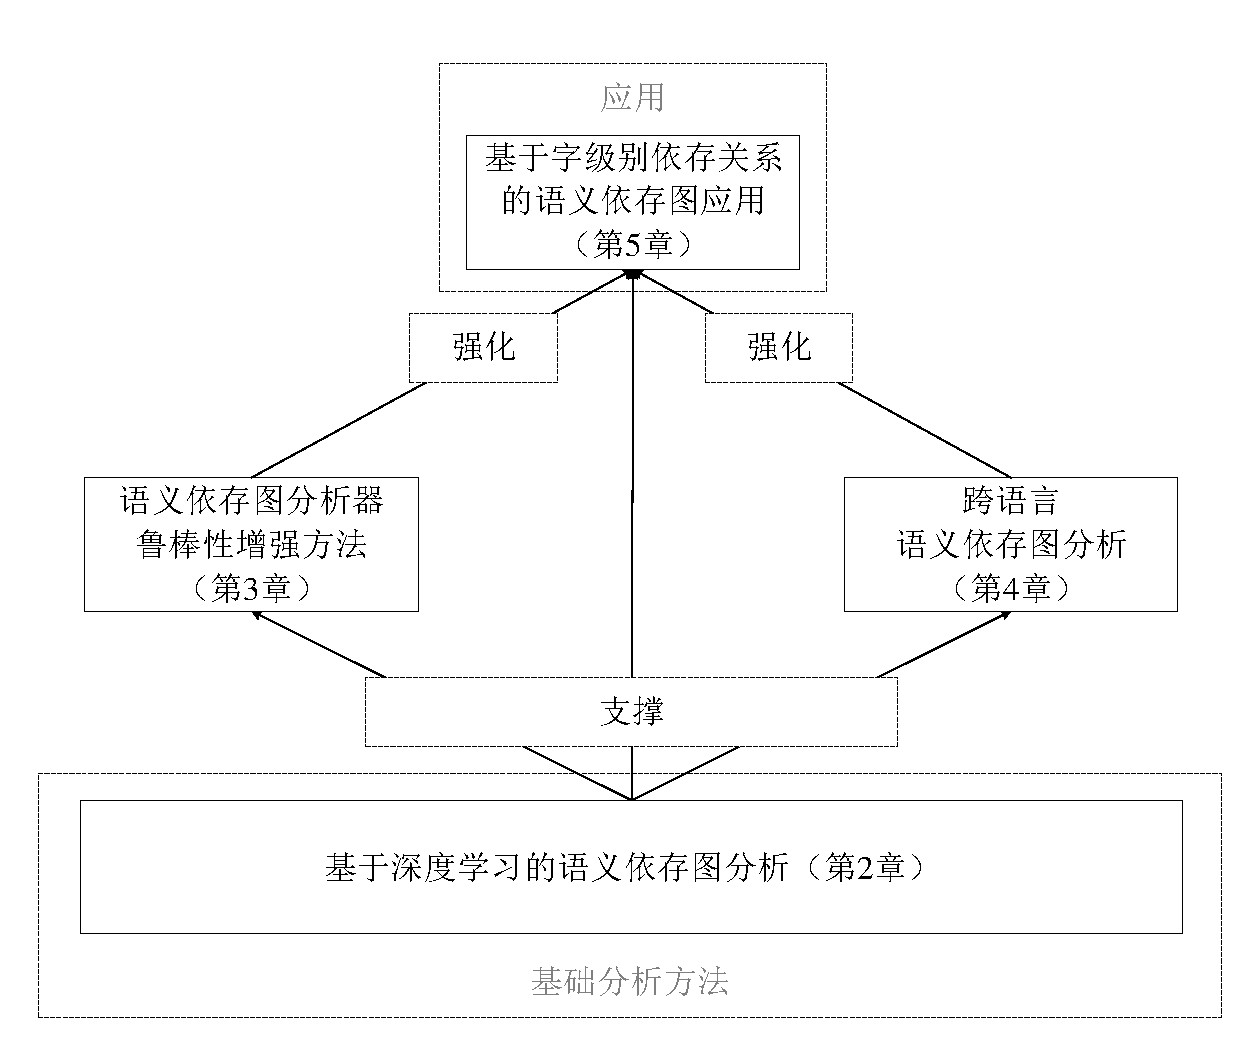
\includegraphics[width=0.95\textwidth]{figures/section-relation.pdf}
    \bicaption[fig:section-relation]{}{论文总体框架}{Fig.$\!$}{Structure of the thesis}
\end{figure}

论文结构框架如图\ref{fig:section-relation}所示,具体来说,本文共包含5章,各章内容组织如下:

在第1章中,本文介绍了中文语义依存图分析的研究背景与意义,并对语义依存图分析的研究现状进行了概述与分析,最后对本文主要内容进行了规划。

在第2章中,针对图结构依存分析的挑战,本文使用基于转移的分析方法,设计了一套用于生成依存图的转移系统,并使用基于栈-长短时记忆网络的模型根据当前转移状态预测下一个转移动作。实验结果表明,本文提出的语义依存图分析方法相比此前的方法取得了显著的性能提升。

在第3章中,针对语义依存图分析在非规范文本上性能远低于规范文本的问题,本文首先设计了一套针对语义依存图分析的对抗样本攻击算法,用于生成使目标语义依存图分析器性能下降的非规范文本。
接着,本文深入探究了对此类非规范文本特征和不同类型分析器的鲁棒性,并在此基础上分别提出了基于对抗样本训练和基于模型融合的方法用于提升现有的依存图分析器的鲁棒性。
实验结果表明,本文提出的对抗样本攻击算法能生成高质量的非规范文本,在它们的帮助下本文有效提升了现有的基于神经网络的依存图分析器的鲁棒性。

在第4章中,针对目前世界上大部分语言上语义依存图语料稀缺,语义依存图分析困难的问题,本文首先对中文语义依存图标注规范进行修改,使其适应多语言场景。
接着,本文提出基于标签转换和图神经网络的方法,首先利用标签转换将现有的多语言大规模通用句法依存语料转换为语义依存图的伪数据,然后使用这些数据和小规模人工标注的语义依存图训练基于图神经网络的编码-解码模型,实现将句法依存语料自动转化为语义依存图语料。
最后,本文使用这些自动转化的语义依存图语料训练跨语言的语义依存图分析器。
实验结果表明,本文提出的跨语言语义依存图分析方法相比于普通的只使用跨语言词向量的方法取得了显著的性能提升。

在第5章中,针对语义依存图分析的应用问题,结合中文的词具有字级别的内部结构的特点,本文提出了基于字级别依存关系的强化预训练模型,将中文语义依存图融合到预训练模型中,从而增强其表示能力。
本文接着使用这种强化的预训练模型获取的词表示作为其他自然语言处理任务的输入,从而提升其性能。
实验结果表明,本文提出的方法显著提升了语义角色标注和关系抽取任务的性能。

% Local Variables:
% TeX-master: "../thesis"
% TeX-engine: xetex
% End: